\subsection{Unfolding the Magic of Folded Dipole Antennas!}

\begin{tcolorbox}[colback=gray!10, colframe=black, title=E9C08] What is a folded dipole antenna?
\begin{enumerate}[label=\Alph*)]
    \item A dipole one-quarter wavelength long
    \item A center-fed dipole with the ends folded down 90 degrees at the midpoint of each side
    \item \textbf{A half-wave dipole with an additional parallel wire connecting its two ends}
    \item A dipole configured to provide forward gain
\end{enumerate} \end{tcolorbox}

\subsubsection{Understanding Folded Dipole Antennas}

A folded dipole antenna is a specialized type of dipole antenna that enhances certain performance characteristics compared to a standard dipole. To better understand this, let's recap some essential concepts in antenna theory:

1. \textbf{Dipole Antenna Basics:}: A standard dipole antenna consists of two conductive elements or arms, typically of equal length and oriented in opposite directions. The length of each arm is usually a half-wavelength of the frequency of operation.

2. \textbf{Folded Design:}: The key feature of a folded dipole is the inclusion of a second wire, parallel to the main element, effectively connecting the ends of the dipole. This configuration results in a higher impedance, which can facilitate better matching with transmission lines and reduce the loss of signal.

3. \textbf{Impedance Matching:}: The standard dipole has an impedance of approximately 73 ohms. By folding the dipole, the impedance increases to about 300 ohms, making it more suitable for use with certain types of feedlines, particularly 300-ohm twin-lead cables.

4. \textbf{Radiation Patterns:}: While the folded dipole maintains a similar radiation pattern to a regular dipole, it can exhibit lower broadside gain in some configurations, making it essential for specific applications where higher gain is not critical.

5. \textbf{Applications:}: Folded dipoles are frequently used in applications such as television antennas and in cases where a more balanced feed is required, especially in high-frequency operations.

\subsubsection{Calculating Antenna Length}

For those looking to understand antenna design further, calculating the length of a dipole is critical. The length \( L \) of a half-wave dipole antenna can be determined using the following formula:

\[
L = \frac{468}{f}
\]

where \( L \) is in feet and \( f \) is the frequency in megahertz (MHz).

For example, if we want to determine the length of a half-wave dipole for a frequency of 144 MHz (typically used in amateur radio), the calculation would be:

\[
L = \frac{468}{144} \approx 3.25 \text{ feet}
\]

Thus, each leg of the dipole should be approximately:

\[
\frac{3.25}{2} \approx 1.625 \text{ feet}
\]

\subsubsection{Visualizing the Folded Dipole}

To aid understanding, a simple diagram illustrating the basic structure of a folded dipole antenna can be constructed using TikZ:

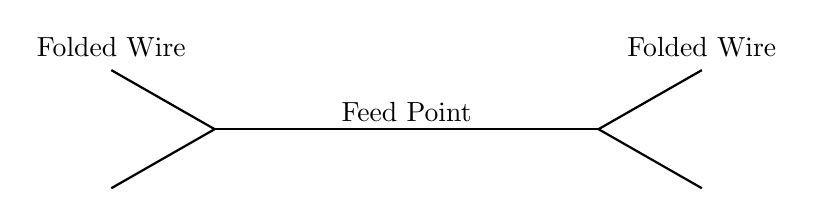
\begin{tikzpicture}[scale=1.5]
    % Draw the main dipole
    \draw[thick] (0, 0) -- (1.625, 0);
    \draw[thick] (-1.625, 0) -- (0, 0);
    % Draw the folded wire
    \draw[thick] (1.625, 0) -- (2.5, 0.5);
    \draw[thick] (1.625, 0) -- (2.5, -0.5);
    \draw[thick] (-1.625, 0) -- (-2.5, 0.5);
    \draw[thick] (-1.625, 0) -- (-2.5, -0.5);
    % Labels
    \node at (0, 0.15) {Feed Point};
    \node at (2.5, 0.7) {Folded Wire};
    \node at (-2.5, 0.7) {Folded Wire};
\end{tikzpicture}
